In this section we follow the work \cite{Burrage2007} to examine the 
stationary density of the Steklov method and determine how close is from the continuous associated stationary 
density. In due so, we consider the SDE
\begin{align}
	dX_t &= V_t dt \label{eqn:SecondOrderSDE1}\\ 
	dV_t &= -\eta s^2(X_t)V_tdt + f(X_t)dt + \varepsilon s(X_t) dW_t.
	\label{eqn:SecondOrderSDE2}
\end{align}
First we will analyze the case when $s(x)= 1$, and $f(x)$ is linear, we will say
$f(x) = -gx$, $g>0$. In this case this SDE reads
\begin{align}
	dX_t &= V_t dt	\label{eqn:LinearSecondOrderSDE1}\\
	dV_t &= -\eta V_tdt -gX_t dt + \varepsilon dW_t.\label{eqn:LinearSecondOrderSDE2}
\end{align}
The stationary density $\mathbb{P}_\infty$  defined as
\begin{equation*}
	\mathbb{P}_\infty = \lim_{t\to \infty}\mathbb{P}(x,v;t)
\end{equation*}
has the following analytical form, independent of the parameters functions of the SDE and sufficiently 
conditions on the potential $V(x)$
\begin{equation*}
	\mathbb{P}_\infty = N \exp\left(
		-\frac{v^2}{2KT} -\frac{V(X)}{KT}
		\right).
\end{equation*}
So, we will compare three quantities, the mean , the variance and covariance of 
the method with the analytical form. If we consider the linear form the SDE 
\crefrange{eqn:SecondOrderSDE1}{eqn:SecondOrderSDE2}
i.e. \crefrange{eqn:LinearSecondOrderSDE1}{eqn:LinearSecondOrderSDE2} then the corresponding stationary distribution is 
Gaussian and 
takes the form
\begin{equation*}
	\mathbb{P}_{\infty}(x,v) = N \exp
	\left(
	-\frac{gx^2}{2KT}
	-\frac{v^2}{2KT}
	\right).
\end{equation*}
Moreover, the solution of \crefrange{eqn:LinearSecondOrderSDE1}{eqn:LinearSecondOrderSDE2} satisfy
\begin{equation*}
	\lim_{t \to \infty} \left\langle X_t^2\right\rangle = \frac{1}{g}KT, \qquad
	\lim_{t \to \infty} \left\langle V_t^2\right\rangle = KT, \qquad
	\lim_{t \to \infty} \left\langle X_t,V_t\right\rangle = 0.
\end{equation*}
Note that SDE \crefrange{eqn:LinearSecondOrderSDE1}{eqn:LinearSecondOrderSDE2} can be written in matrix notation as
\begin{equation}
	d 
	\begin{bmatrix}
		X_t\\ V_t
	\end{bmatrix}
	=
	Q
	\begin{bmatrix}
			X_t\\ V_t
	\end{bmatrix}
	+ \varepsilon
	\begin{bmatrix}
			0\\ 1
	\end{bmatrix}
	dW_t
\end{equation}
	where
$$
	Q =
\begin{bmatrix}
	0	& 1	\\
	-g	& -\eta	\\
\end{bmatrix}
$$
In this way, we consider numerical updates of the form
\begin{align}\label{eqn:NumericalUpdate}
	&\begin{bmatrix}
		X_{n+1}\\ V_{n+1}
	\end{bmatrix}
	=
	R
	\begin{bmatrix}
		X_{n}\\ V_{n}
	\end{bmatrix}
	+ \varepsilon r \Delta W_n\\
	&R =
	\begin{bmatrix}
		r_{11}	& r_{12}\\
		r_{21}	& r_{22}\\
	\end{bmatrix},
	\qquad 
	r=
	\begin{bmatrix}
		r_1\\
		r_2
	\end{bmatrix}
\end{align}
Since the numerical update \eqref{eqn:NumericalUpdate} is linear in $W_n$ the stationary discrete density 
$\mathbb{P}_{\infty}^{*}(x,v)$ is Gaussian. We take the correlation matrix 
$$
	\Sigma=
	\begin{bmatrix}
		\sigma_x^2,	& \mu\\
		\mu			& \sigma_v^{2}
	\end{bmatrix}
$$
where
\begin{equation}
	\sigma_x^2 = \lim_{n \to \infty} \left\langle X_n^2\right\rangle, \qquad
	\sigma_v^2 = \lim_{n \to \infty} \left\langle V_n^2\right\rangle, \qquad
\mu = \lim_{n \to \infty} \left\langle X_n,V_n\right\rangle .
\end{equation}
Then
\begin{equation}
	\mathbb{P}_{\infty}^* = 
		\frac{1}{2\pi}
		\left|
			\Sigma^{-1}
		\right|^{\frac{1}{2}}
	\exp\left(
		-\frac{1}{2}(x,v)
		\Sigma^{-1}
		\begin{bmatrix}
			x\\v
		\end{bmatrix}
	\right).
\end{equation}
This stationary density has the property of invariance under the linear transformation 
\eqref{eqn:NumericalUpdate}, thus the correlation matrix that results from a numerical method 
satisfies
\begin{equation}
	R \Sigma R^T = \Sigma - \varepsilon^2 r r^T \Delta t.
\end{equation}
Since $\Sigma$ is simetric we can rewrite this equation in a inversion suitable form as
\begin{equation}\label{eqn:MatrixEquation}
	\begin{bmatrix}
		r_{11}^2 - 1	&2r_{11}r_{12}						&r_{12}^2		\\
		r_{11}r_{12}	&r_{11}r_{12}+ r_{12}r_{21} - 1		&r_{11}r_{12}	\\
		r_{21}^2		&2r_{11}r_{12}						&r_{22}^2 -1
	\end{bmatrix}
	\begin{bmatrix}
		\sigma_x^2\\
		\mu\\
		\sigma_v^2
	\end{bmatrix}
	= -\varepsilon^2
	h
	\begin{bmatrix}
		r_1^2\\
		r_1 r_2\\
		r_2^2
	\end{bmatrix}.
\end{equation}
Then solving \cref{eqn:MatrixEquation} we found the stability boundaries of the method  as function
of the parameters $\eta h $, $g h^2$.
For the SSLS method we can write in matrix form the update of the scheme as follows
\begin{equation}
	\begin{bmatrix}
		X_{n+1}\\
		V_{n+1}
	\end{bmatrix}
	=
	\begin{bmatrix}
		1											& h\\
		\frac{g}{\eta}\left(\exp(-h\eta) - 1 \right)	
		& \exp(-\eta h)% + \frac{g}{\eta}\left(\exp(-h\eta) - 1 \right) h 
	\end{bmatrix}
	\begin{bmatrix}
		X_n\\V_n
	\end{bmatrix}
	+
	\varepsilon
	\begin{bmatrix}
		V_n\\
		X_n
	\end{bmatrix}.
\end{equation}
%
Then equation \eqref{eqn:MatrixEquation} reads
\begin{equation}
	\begin{bmatrix} 
		0	&2h		&{h}^{2}\\ 
		\frac{g}{\eta}
			\left( 
				e^{-\eta h}-1 
			\right)
		&
		e^{-\eta h} 
			+\frac{gh}{\eta}
				\left( 
					e^{-\eta h}-1 
				\right) -1
			&
			h  e^{-\eta h}
			\\ 
		\frac{g^2}{\eta^2} 
			\left( 
				e^{-\eta h}-1
			\right)^2
			&
		\frac{2 g}{\eta}
			\left(
				e^{-\eta h} - 1 
			\right)
			e^{-\eta h}
		& 
		e^{-2\eta h} -1
	\end{bmatrix}
	\begin{bmatrix}
		\sigma_x^2\\
		\mu\\
		\sigma_v^2
	\end{bmatrix}
	=
	\begin{bmatrix}
		0\\
		0\\
		\epsilon^2 h
	\end{bmatrix}.
\end{equation}
Hence, solving we get
\begin{equation}
	\begin{bmatrix}
		\sigma_x^2\\
		\mu\\
		\sigma_v^2
	\end{bmatrix}
	=
	\frac{2 K T  \eta^3}
	{
		\left( \eta-g h \right)
		\left(e^{-\eta h}-1 \right) 
		\left( 
			2 e^{-\eta h}\eta
			-gh e^{-\eta h}
			+gh
			+2 \eta
		\right)
	}
	\begin {bmatrix}
		\frac{
			\left(
			 e^{-\eta h}\eta
				-gh e^{-\eta h}
				+gh
				+\eta 
			\right)
		}{
			g ( e^{-\eta h}-1)
		}\\ 
		h^2\\ 
		-2h
	\end {bmatrix}.
\end{equation}
Comparing with the correlation matrix for the Euler-Maruyama method 
\begin{equation}
	\Sigma_E = 
	\frac{KT}{1-\frac{g}{\eta}h}
	\left(
		2-\eta h +\frac{1}{2} g h^2
	\right)^{-1}
	\begin{bmatrix}
		g^{-1}(2-\eta h +g h^2) & -h\\
		-h &	2
	\end{bmatrix}
\end{equation}
we can see that the correlation between $X_t$,$ V_t$ is ${o}(h)$ while that for the SSLS is 
$o(h^2)$. In \Cref{fig:MeanSquareEta} we show the difference between the exact and the theoretically 
moments of the Euler and SSLS methods.
\begin{figure}[htb]
	\centering
	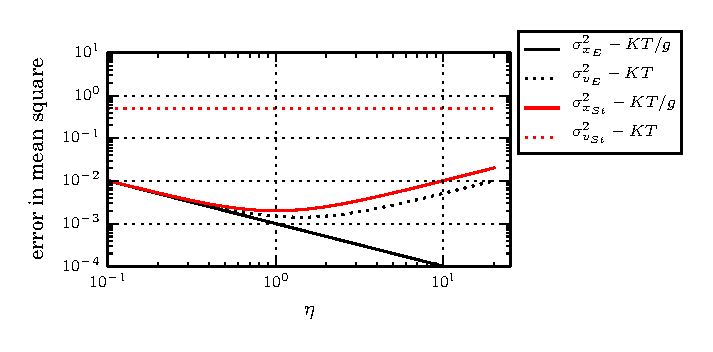
\includegraphics{./papers/paperB/figures/ErrorVariances.eps}
	% ErrorVariances.eps: 0x0 pixel, 300dpi, 0.00x0.00 cm, bb=0 0 256 158
	\caption{Difference between the calculated moments and analytical form versus $\eta$ parameter. Here
	$g=1$, $K = 1$,$T = 1$, and $h =\num{0.1}$.}
	\label{fig:MeanSquareEta}
\end{figure}
